\documentclass[12pt, a4paper]{article}

\usepackage{graphicx,amsmath,amssymb,amsthm, boxedminipage, bm}
\usepackage{float}
\usepackage[body={17cm, 24.62cm}, centering, dvipdfm]{geometry}

\newtheorem{theorem}{Theorem}%[section]
\newtheorem{proposition}[theorem]{Proposition}
\newtheorem{lemma}[theorem]{Lemma}
\newtheorem{corollary}[theorem]{Corollary}
\newtheorem{definition}[theorem]{Definition}

\newcommand{\scalar}[2]{\ensuremath{\langle #1, #2\rangle}}
\newcommand{\floor}[1]{\left\lfloor #1 \right\rfloor}
\newcommand{\ceil}[1]{\left\lceil #1 \right\rceil}
\newcommand{\norm}[1]{\|#1\|}
\newcommand{\pfrac}[2]{\left(\frac{#1}{#2}\right)}
\newcommand{\nth}[1]{#1^{\textsuperscript{th}}}


\newcommand{\N}{\mathbb{N}}
\newcommand{\R}{\mathbb{R}}
\newcounter{exercise}
\newcommand{\exercise}{\addtocounter{exercise}{1}\noindent\textbf{Exercise \arabic{section}.\arabic{exercise}. }}


\usepackage{bm}
\usepackage{longtable}
\usepackage{harpoon}
\usepackage{fontspec}
\usepackage{listings}
\usepackage{setspace}
\usepackage{cmap}
\usepackage{cite}
\usepackage{float}
\usepackage{xeCJK}
\usepackage{amsthm}
\usepackage{amsmath}
\usepackage{amssymb}
\usepackage{setspace}
\usepackage{enumerate}
\usepackage{indentfirst}
\usepackage{algorithm}
\usepackage{algpseudocode}
\usepackage{diagbox}
\usepackage[colorlinks]{hyperref}
\usepackage[short,nodayofweek,level,24hr]{datetime}

\usepackage[table]{xcolor}
\usepackage{booktabs}
\usepackage[cache=false]{minted}
\usepackage{pdfpages}
\usepackage{tikz}
\allowdisplaybreaks

%\setlength{\parindent}{0em}
%\setlength{\mathindent}{0pt}
\algnewcommand\AND{\textbf{and~}}
\algnewcommand\OR{\textbf{or~}}
\newfontfamily\Courier{Courier New}
\renewcommand{\theFancyVerbLine}{\rmfamily\scriptsize\arabic{FancyVerbLine}}
\newcommand{\cppcode}[1]{
    \inputminted[mathescape,
    			 tabsize=4,
    			 framesep=2mm,
    			 breakaftergroup=true,
    			 breakautoindent=true,
    			 breakbytoken=true,
    			 breaklines=true,
    			 fontsize=\small
    ]{cpp}{#1}
}
\newcommand{\javacode}[1]{
    \inputminted[mathescape,
    			 tabsize=2,
    			 linenos,
    			 frame=single,
    			 framesep=2mm,
    			 breakaftergroup=true,
    			 breakautoindent=true,
    			 breakbytoken=true,
    			 breaklines=true,
    			 fontsize=\small
    ]{java}{#1}
}
\newcommand{\pythoncode}[1]{
    \inputminted[mathescape,
    			 tabsize=2,
    			 linenos,
    			 breakaftergroup=true,
    			 breakautoindent=true,
    			 breakbytoken=true,
    			 breaklines=true,
    			 fontsize=\small
    ]{python}{#1}
}
\newcommand{\vimcode}[1]{
    \inputminted[mathescape,
    			 tabsize=2,
    			 linenos,
    			 frame=single,
    			 framesep=2mm,
    			 breakaftergroup=true,
    			 breakautoindent=true,
    			 breakbytoken=true,
    			 breaklines=true
    			 fontsize=\small
    ]{vim}{#1}
}
\setcounter{section}{1}
\begin{document}
	\title{CS217 - Algorithm Design and Analysis\\Homework Assignment 2}
	\author{
		\begin{tabular}{rl}
		    \textbf{Group Name:\,\,\,\,\,\,\,\,\,\,}& Static\\
		    \textbf{Group Members: }& Zhenjia Xu, JiaCheng Yang\\
			& Zhuolin Yang, Wenda Qiu
		\end{tabular}
	}
	\date{\today}
	\maketitle
	\section{Sorting Algorithms}
	\exercise{}\begin{proof}
	Because $X \cup \{e\}$ is good, there exists a minimum spanning tree $T$ of $G$ such that $X \cup \{e\}~\subseteq~E(T)$.
	In this spanning tree $T$, $\{e\}$ connects two components, denoted by $S, V \setminus S$. \\
	Consider the cut of G: $S, V \setminus S$.
	\begin{enumerate}[(i)]
		\item Obviously, for each edge $e(u,v)$ in $X$, either $u,v~\in~S$ holds or $u,v~\in~V\setminus S$ holds; that is to say it can't crosss the cut.
		\item If $e$ is't a minimum weight edge of $G$ crossing this cut; that is to say, there exist a smaller edge crossing $G$, denoted by $e'$.\\
			Then $T\setminus\{e\} \cup \{e'\}$ forms a smaller spanning tree, which contradicts the condition that $T$ is the minimum spanning tree.\\
			So $e$ is a minimum weight edge of $G$ crossing this cut.
	\end{enumerate}
\end{proof}

	\exercise{}\begin{itemize}
	\item Step1, Let $B_0 = A$ ($B_0$ is of size $n$).
	\item Step2, divide $B_0$ into $n/2$ pairs, make a comparison in each pair and put the bigger one into $B_1$ ($B_1$ is of size $n/2$).
	\item Step3, do the similar thing in Step2 to generate $B_2$ by $B_1$, generate$B_3$ by $B_2 \cdots$ until we get $B_{\log_{2}n}$(containing only one element, which is the maximum).
\end{itemize}

\indent The above three steps use $n - 1$ comparisons in all.

Because we need $\displaystyle \frac{n}{2^i}$ comparions to generate $B_i (1\leq i \leq \log_{2}n)$
\[\sum_{i = 1} ^ {\log_{2}n} \frac{n}{2^i}= n - 1\]

The maximum element compares with $\log_{2}n$ elements in above steps, and the second largest element is obviously in these $\log_{2}n$ elements. So we only need another $\log_{2}n - 1$ comparisons to find the second largest element.

In all, the total number of comparisons is $N = n - 1 + \log_{2}n - 1 = n + \log_{2}n - 2$

	
	\exercise{}The additions we need is the same as Exercise2, $k\cdot (n-k+1)$.
But this time the addition can be done in $O(1)$ time because we only need to keep the result modulo $2$.
So the running time is $O(k\cdot (n-k+1))$.
The input size is $O(\log n)$ and the output size is $O(1)$. It is not an efficient algorithm comparing to the input/output size.


	\exercise{}\begin{enumerate}[(1)]
\item
	Transfer vertex capacities into edge capacities:
	\begin{itemize}
		\item Divide each vertex $u \in V$ into two vertexes, denoted by $u_{in}$ and $u_{out}$. Connect an edge from $u_{in}$ to $u_{out}$ with a capacity of $c$
		\item For each edge $\langle u, v \rangle \in E$, connect an edge from $u_{out}$ to $v_{in}$ with a capacity of $\infty$
		\item Calculate the maximum flow from $S_{in}$ to $T_{out}$
	\end{itemize}

	Transfer edge capacities into vertex capacities:
	\begin{itemize}
		\item For each vertex $u \in V$, still construct a vertex $v$ in $V'$ with a capacity of $\infty$
		\item For each edge $e\langle u, v, c\rangle \in E$, construct a vertex $p_e$ with a capacity of c, and connect edges from $u$ to $p_e$ and from $p_e$ to $v$
		\item Calculate the maximum flow from $S$ to $T$
	\end{itemize}
	\item Illustration

	The black edge's capacity is $\infty$, the red edge's capacity is $c$

	The black vertex's capacity is $\infty$, the red vertex's capacity is $c$

	These two pictures show Transfering vertex capacities into edge capacities.
	\begin{figure}[!htbp]
		\centering
		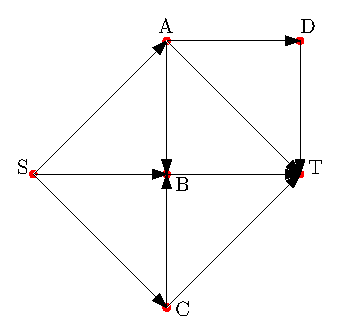
\includegraphics[totalheight=6cm]{source/xzj/pic1.eps}
		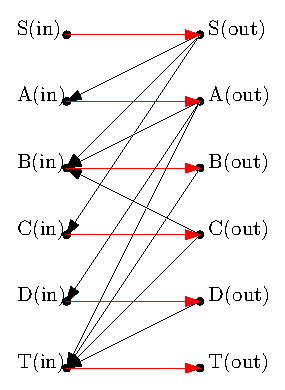
\includegraphics[totalheight=6cm]{source/xzj/pic2.eps}
	\end{figure}
	These two pictures show Transfering edge capacities into vertex capacities.
	\begin{figure}[!htbp]
		\centering
		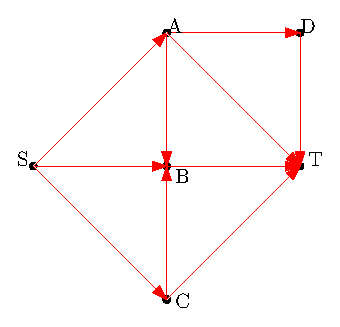
\includegraphics[totalheight=6cm]{source/xzj/pic3.eps}
		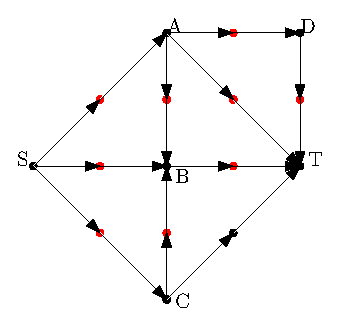
\includegraphics[totalheight=6cm]{source/xzj/pic4.eps}
	\end{figure}

	\item Construct a vertex capacities network $G = (V, E, c)$. The $c$ of $s$ and $t$ is $\infty$, and for other vertics, $c$ is $1$.
	Calculate the maximum flow from $s$ to $t$.
	Each flow from $s$ to $t$ represent a path from $s$ to $t$.
	Because the vertex capacities are 1 (except for $s, t$), these paths are internally vertex disjoint.
	There $k$ paths from $s$ to $t$, such that the paths are internally vertex disjoint if and only if the maximum flow if no less than $k$.
\end{enumerate}


	\exercise{}We can easily come out an algorithm using the formular which is proved in Ex5.
\begin{algorithm}[H]
	\caption{An efficient method calculating the binomial coefficient}
	\begin{algorithmic}[1]
		\Function {binom} {$n$, $k$, $p$}
			\If {$m > n$ \OR $m < 0$}
				\State \Return $0$
			\EndIf
			\If{$n < 2$} :
				\State \Return $1$
			\EndIf
			\If{$p = 0$} :
				\State $p = 1$
				\While{$p * 2 \geq n$}
					\State $p \leftarrow p * 2$
				\EndWhile
			\Else
				\While{$p \geq n$}
					\State $p \leftarrow p / 2$
				\EndWhile
			\EndIf
			\State \Return (\Call{Binom}{$n - p$, $m - p$, $p$} + \Call{Binom}{$n - p$, $m$, $p$}) $\bmod 2$
		\EndFunction
	\end{algorithmic}
\end{algorithm}

\noindent The implementation in python is displayed below
\pythoncode{source/xzj/ex5.py}


	\exercise{}\subsubsection*{FLGV}
According to \textbf{FLGV-2}, we have:
\[\exists \textbf{y} \in \textbf{R}^{m}: A^{T}\textbf{y} \geq 0, \textbf{b}^{T}\textbf{y} < 0 \]
if FLGV-1 also holds, there exists $\textbf{x} \geq 0$, $A\textbf{x}=\textbf{b}$.
\noindent
because $A\textbf{x}=\textbf{b}$ can be written as $\textbf{b}^{T} = \textbf{x}^{T}A^{T}$, we have:
\[\textbf{b}^{T}\textbf{y}=\textbf{x}^{T}A^{T}\textbf{y}\]
Because $A^{T}\textbf{y} \geq 0$, $\textbf{x} \geq 0$, we can get $\textbf{x}^{T}A^{T}\textbf{y} \geq 0$. But according to \textbf{FLGV-2}, $\textbf{b}^{T}\textbf{y} < 0$, which is a contradictory, so FLGV-2 implies that \textbf{FLGV-1} does not hold.
\subsubsection*{FLLPV}
According to \textbf{FLLPV-2}, we have:
\[\exists \textbf{y} \in \mathbb{R}^{m}: \textbf{y} \geq 0, A^{T}\textbf{y} \geq 0, \textbf{b}^{T}\textbf{y} < 0 \]
if \textbf{FLLPV-1} also holds, there exists $\textbf{x} \geq 0$, $A\textbf{x} \leq \textbf{b}$. Because $A\textbf{x} \leq \textbf{b}$ can be written as $\textbf{b}^{T} \geq \textbf{x}^{T}A^{T}$, and $\textbf{y}$ holds $\textbf{y} \geq 0$, we have:
\[\textbf{b}^{T}\textbf{y} \geq \textbf{x}^{T}A^{T}\textbf{y}\]
Because $A^{T}\textbf{y} \geq 0$, $\textbf{x} \geq 0$, we can get $\textbf{b}^{T}\textbf{y} \geq \textbf{x}^{T}A^{T}\textbf{y} \geq 0$.
But according to \textbf{FLLPV-2}, $\textbf{b}^{T}\textbf{y} < 0$, which is a contradictory, so \textbf{FLLPV-2} implies that FLLPV-1 does not hold.
\subsubsection*{FLEV}
According to \textbf{FLEV-2}, we have:
\[\exists \textbf{y} \in \mathbb{R}^{m}: \textbf{y} \geq 0, A^{T}\textbf{y} \geq 0, \textbf{b}^{T}\textbf{y} < 0 \]
If \textbf{FLEV-1} also holds, there exists $A\textbf{x} \leq \textbf{b}$.
Because $A\textbf{x} \leq \textbf{b}$ can be written as $\textbf{b}^{T} \geq \textbf{x}^{T}A^{T}$, and $\textbf{y}$ holds $\textbf{y} \geq 0$, we have:
\[\textbf{b}^{T}\textbf{y} \geq \textbf{x}^{T}A^{T}\textbf{y}\]
Because $A^{T}\textbf{y} \geq 0$, $\textbf{x} \geq 0$, we can get $\textbf{b}^{T}\textbf{y} \geq \textbf{x}^{T}A^{T}\textbf{y} \geq 0$.
But according to \textbf{FLEV-2}, $\textbf{b}^{T}\textbf{y} < 0$, which is a contradictory, so \textbf{FLEV-2} implies that FLEV-1 does not hold.


	\exercise{}Let's define $[i, j]$ as a set which contains the integral numbers between $i$ and $j$.
Recalling the proof that $A_{i, j} = 1$ iff the number in $[i, j]$ in the input sequence that occurs first must be $i$, we can obvirusly make an inferrence that $B_{i, j, k} = 1$ iff the number in $[i, j] \cup [i, k]$ in the input sequence that occurs first must be $i$.

Notice that every number has no difference among other numbers except their pronunciations. In other words, we can choose the number which occurs first with equal probability.

Hence
\[\mathbb{E}[B_{i, j, k}] = \dfrac{1}{\left|[i, j] \cup [i, k]\right|}\]

\begin{lemma}
$\left|[i, j] \cup [i, k]\right| = \max\{i, j, k\} - \min\{i, j, k\} + 1$
\end{lemma}
\begin{proof}
We will prove the lemma with three cases below.
\begin{itemize}
\item If $i = \min\{i, j, k\}$, then
\[\left|[i, j] \cup [i, k]\right| = \max\{j, k\} - i + 1 = \max\{i, j, k\} - \min\{i, j, k\} + 1\]
\item If $i = \max\{i, j, k\}$, then
\[\left|[i, j] \cup [i, k]\right| = i - \min\{j, k\} + 1 = \max\{i, j, k\} - \min\{i, j, k\} + 1\]
\item If $j < i < k$ or $k < i < j$, then
\[\left|[i, j] \cup [i, k]\right| = \max\{j, k\} - \min\{j, k\} + 1 = \max\{i, j, k\} - \min\{i, j, k\} + 1\]
\end{itemize}
\end{proof}

According to the lemma, the following formula holds.
\[\mathbb{E}[B_{i, j, k}] = \dfrac{1}{\max\{i, j, k\} - \min\{i, j, k\} + 1}\]

	
	\exercise{}Suppose that there are two different minimum spanning tree, called $T,T'$.\par

We can find the edge which belongs to only one of the minimum spanning tree and its weight is minimal.
Because no two edges of $G$ have the same weight, the above edge is unique, denoted as $e$.
(Without loss of generality, let $e$ belong to $T$)\par

By Lemma 3, we known that \[m_{c_e}\{T\} = m_{c_e}\{T'\}~\text{and}~m_{c_e - 1}\{T\} = m_{c_e - 1}\{T'\}\]
So \[m_{c_e}\{T\} -  m_{c_e - 1}\{T\} = m_{c_e}\{T'\} - m_{c_e - 1}\{T'\}\]
However, $e$ belongs to only $T$, in other word \[m_{c_e}\{T\} -  m_{c_e - 1}\{T\} = 1~\text{and}~ m_{c_e}\{T'\} - m_{c_e - 1}\{T'\} = 0\] which contradicts the equation above.\par
So, the hypothesis is wrong; that is to say $G$ has only one minimum spanning tree.


	\exercise{}\section{Ex.9}
	As we did in Ex8, let $k$ be the answer for $QUICKSELECT$. Since the input is random, we can assume that every number from $1$ to $n$ is equally likely to be the answer.\par
	So the expected number of comparisons is
	\begin{align*}
		E[C] &= \frac{1}{n}\sum_{k=1}^{n}E[\sum_{i\neq j, i\neq k, j\neq k}B_{i,j,k}+\sum_{i\neq k}A_{k,i}]\\
		&= \frac{1}{n}(\sum_{i\neq j, i\neq k, j\neq k}\frac{1}{\max(i,j,k)-\min(i,j,k) + 1} + \sum_{i\neq k}\frac{1}{|i-k|+1})\\
	\end{align*}
		$\sum_{i\neq k}\frac{1}{|i-k|+1}$ is calculated in Ex5 : $$\sum_{i\neq k}\frac{1}{|i-k|+1}=2(n+1)H_n-4n$$\par
		Now we calculate the other part :
	\begin{align*}
		\sum_{i\neq j, i\neq k, j\neq k}\frac{1}{\max(i,j,k)-\min(i,j,k) + 1} &= 3!\sum_{L=3}^{n}\frac{\binom{1}{n-L+1}\binom{1}{L-2}}{L}\\
		&= 6\sum_{L=3}^{n}\frac{(n+3)L-L^2-2(n+1)}{L}\\
		&= 21n+3n^2-12H_n-12nH_n\\
	\end{align*}
	where $L$ is $\max(i,j,k)-\min(i,j,k)+1$.\par
	Then we have :
	\begin{align*}
			E[C] &= \frac{21n+3n^2-12H_n-12nH_n+2(n+1)H_n-4n}{n}\\
			&= 3n-10H_n-\frac{10H_n}{n}+17\\
	\end{align*}
\end{document}
